\documentclass{article}
\usepackage{graphicx}
\usepackage{amsmath}%
\setcounter{MaxMatrixCols}{30}%
\usepackage{amsfonts}%
\usepackage{amssymb}%
\title{Google Reactor Calibration Model}
\author{Jin Liu}
%\date{February 21, 2017}
\setlength\parindent{0pt}
\begin{document}
\maketitle

This note is to describe the parameters and formula Google IPB Reactor Calibration Model.\\
\\

The proposed equivalent circuit model is described in Figure 1.\\

\begin{figure}
[h]
\begin{center}
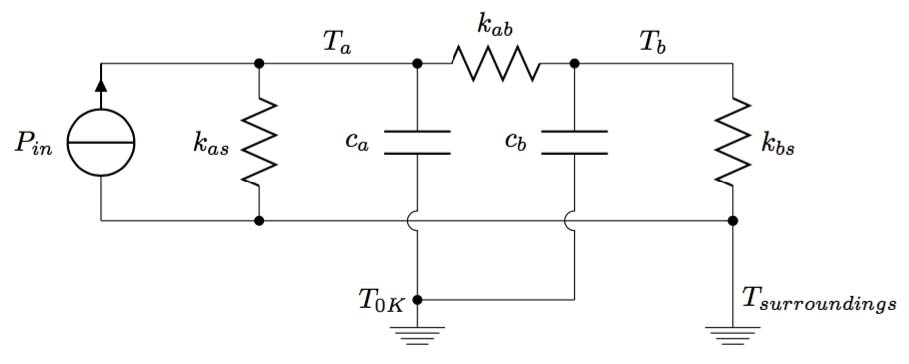
\includegraphics[scale=1]{formula1.jpg} 
\caption{Circuit Model}%
\end{center}
\end{figure} 
The governing equations are:
\begin{equation}
\frac{dT_{a}(t)}{dt}=\frac{P_{in}-k_{as}(T_{a}-T_{s})-k_{ab}(T{a}-T_{b})}{c_{a}}\label{1}%
\end{equation} 

\begin{equation}
\frac{dT_{b}(t)}{dt}=\frac{P_{in}-k_{ab}(T_{a}-T_{s})-k_{bs}(T{b}-T_{s})}{c_{b}}\label{1}%
\end{equation} 

The parameters in the equations are:
\begin{equation}
k_{as}=(k_{as0}+k_{as1}T_{a}+k_{as2}T_{a}^{2})\label{1}%
\end{equation}  
\begin{equation}
k_{ab}=(k_{ab0}+k_{ab1}T_{a}+k_{ab2}T_{a}^{2})
\end{equation}  
\begin{equation}
k_{bs}=(k_{bs0}+k_{bs1}T_{b}+k_{bs2}T_{b}^{2})
\end{equation}  
\begin{equation}
c_{a}=(c_{a0}+c_{a1}T_{a}+c_{a2}T_{a}^{2})
\end{equation}  
\begin{equation}
c_{b}=(c_{b0}+c_{b1}T_{b}+c_{b2}T_{b}^{2})
\end{equation} 

\begin{equation}
P_{in}(t)=(a_{10}+a_{11}T_{a}+a_{12}T_{a}^{2})P_{heaterpower} + (a_{20}+a_{21}T_{a}+a_{22}T_{a}^{2})P_{core-Q}\label{1}%
\end{equation}
in $DC$ $P_{core-Q}$ is $P_{DC}$\\

$T_{a}$ is the core temperature\\
$T_{b}$ is the inner block temperature\\
$T_{s}$ is the outer block temperature\\

\begin{equation}
P_{out}(t)=k_{as}[T_{a}(t)-T_{s}(t)]+k_{bs}[T_{b}(t)-T_{s}(t)]\label{1}%
\end{equation}  

\begin{equation}
P_{stored}(t)=c_{a}\frac{dT_{a}(t)}{dt}+c_{b}\frac{dT_{b}(t)}{dt}\label{1}%
\end{equation}  

The Energy COP defined as
\begin{equation}
COP_{energy}(t)=\frac{\int_{0}^{t}{[P_{out}(t)+P_{stored}(t)]dt}}{\int_{0}^{t}P_{in}(t)dt}\label{1}%
\end{equation}

The Power COP defined as

\begin{equation}
COP_{power}(t)=\frac{{P_{out}(t)+P_{stored}(t)}}{P_{in}(t)}\label{1}%
\end{equation}

The Google Team has done four calibration models, the table 1. lists all the parameters in the calibration models.
\begin{table}[h]
\centering
\caption{Parameters in Google Model}

\begin{tabular}{|c|c|c|c|c|}
\hline
Parameters & ipb1-30b-he & ipb1-30b-h2 & sri-ipb2-27b-h2 & sri-ipb2-33b-he\\ \hline
ca0	&	10.58	&	52.91	&	17.19	&	20.59	\\	\hline
ca1	&	0.4303	&	0.2200	&	-0.6768	&	0.0857	\\	\hline
ca2	&	-0.0009	&	-0.0003	&	0.0086	&	0.0000	\\	\hline
cb0	&	601.10	&	579.90	&	883.48	&	675.09	\\	\hline
cb1	&	0.4669	&	0.3826	&	-2.7510	&	0.1209	\\	\hline
cb2	&	0.0000	&	0.0000	&	0.0000	&	0.0000	\\	\hline
kas0	&	0.0292	&	0.0266	&	0.0001	&	0.0017	\\	\hline
kas1	&	-0.0001	&	0.0000	&	0.0002	&	0.0000	\\	\hline
kas2	&	0.0000	&	0.0000	&	0.0000	&	0.0000	\\	\hline
kab0	&	0.6535	&	0.6192	&	0.8300	&	0.5686	\\	\hline
kab1	&	-0.0005	&	0.0008	&	-0.0024	&	0.0008	\\	\hline
kab2	&	0.0000	&	0.0000	&	0.0000	&	0.0000	\\	\hline
kbs0	&	0.0330	&	0.0368	&	0.0753	&	0.0637	\\	\hline
kbs1	&	0.0002	&	0.0001	&	-0.0003	&	0.0001	\\	\hline
kbs2	&	0.0000	&	0.0000	&	0.0000	&	0.0000	\\	\hline
a10	&	1.0000	&	1.0000	&	1.0000	&	1.0000	\\	\hline
a11	&	0.0000	&	0.0000	&	0.0000	&	0.0000	\\	\hline
a12	&	0.0000	&	0.0000	&	0.0000	&	0.0000	\\	\hline
a20	&	0.3676	&	0.3598	&	0.4250	&	0.0505	\\	\hline
a21	&	0.0010	&	0.0007	&	-0.0009	&	0.0031	\\	\hline
a22	&	0.0000	&	0.0000	&	0.0000	&	0.0000	\\	\hline

\end{tabular}
\end{table}

\end{document}
